% File:		vec-2d.tex
% Author:	See Below
% Date:	        See Below
%
% The authors have placed this file in the public domain;
% they make no warranty and accept no liability for this file.

\documentclass[12pt]{article}
\usepackage{times}
\usepackage{color}
\usepackage[usenames]{xcolor}
\usepackage{scalefnt}
\usepackage{tikz}
\usepackage{wrapfig}
\usetikzlibrary{arrows}
\begin{document}
\newcommand{\header}[1]{\underline{\bf #1}}
\newcommand{\file}[1]{{\bf #1}}
\newcommand{\blankpage}{\newpage\vspace*{3.5in}%
    \centerline{\Large This Page is Intentionally Left Blank}}
\setlength{\parindent}{0.0in}
\setlength{\parskip}{1ex}
\newcommand{\key}[1]{{\bf #1}}
\newcommand{\TT}[1]{{\tt \bfseries #1}}
\newcommand{\EOL}{\penalty \exhyphenpenalty}
\newtheorem{definition}{Definition}[section]
\newtheorem{lemma}{Lemma}[section]
\newenvironment{indpar}[1]%
    {\begin{list}{}{\setlength{\leftmargin}{#1}}\item[]}%
    {\end{list}}

\section{Two Dimensional Vector Calculator}
This document describes a group of problems involving 2-dimensional vectors,
starting with simple vector calculations, and working up to polygons.
The problems are embedded in a simple calculator for ease of
testing.

\section{Boolean, Scalars, Vectors, and Transforms}
A \key{boolean} here is either the symbol \key{true} or the symbol \key{false}.

A \key{scalar} here is a double precision floating point number.

A \key{vector} here is a pair $(x,y)$ of double precision floating point
numbers, $x$ denoting an X-coordinate value, and $y$ denoting a
Y-coordinate value.  Such a vector can denote a point $(p_x,p_y)$ in the
XY-plane, or can denote a translation $v$ of the plane:
\centerline{$(p_x,p_y) \longmapsto (p_x+v_x,p_y+v_y)$}

The product of a scalar $s$ and a vector $v=(v_x,v_y)$ is represented using
$*$ as $s*v == (sv_x,sv_y)$.

A \key{linear transformation} here is a pair of vectors, $(\ell_x,\ell_y)$
representing the map:
\centerline{$(v_x,v_y) \longmapsto v_x*\ell_x+v_y*\ell_y$}
Application is represented using
$*$ as $(\ell_x,\ell_y)*v=v_x*\ell_x+v_y*\ell_y$.

An \key{affine transformation} here is a triple of vectors,
$(\ell_x,\ell_y,\tau)$
representing: \\
\centerline{$(v_x,v_y) \longmapsto v_x*\ell_x+v_y*\ell_y+\tau$}
Application is represented using
$*$ as $(\ell_x,\ell_y,\tau)*v=v_x*\ell_x+v_y*\ell_y+\tau$. \\
(An affine transformation is a linear transformation followed by
a translation.)

\newpage

\section{The Calculator Language}
The calculator language of this problem is very simple.
An example is:
\\[1ex]
{\tt
\hspace*{0.2in}\begin{tabular}{l@{\hspace{0.5in}}l}
\rm \bf Input	& \rm \bf Output \\\hline
x=4		& x=4 \\
y = 0.5         & y = 0.5 \\
z = x + y       & z = x + y = 4.5 \\
v=(3,-2)	& v=(3,-2) \\
w=z*v		& w=z*v = (13.5,-9) \\
\# this is a comment & \# this is a comment
\end{tabular}
} % \tt

The syntax is:
\\[1ex]
\hspace*{0.2in}\begin{tabular}{l}
{\em program} ::= {\em statement}$^\star$ \\
{\em statement} ::= \\
\hspace*{0.2in}\begin{tabular}[t]{cl}
                    & {\em comment} \\
                $|$ & {\em variable} \TT{=} {\em value} {\em eol}\\
                $|$ & {\em variable} \TT{=} {\em operator}
		          {\em variable} 
		          {\em operator}$^?$ {\em eol} \\
                $|$ & {\em variable} \TT{=} {\em variable} {\em operator}
		          {\em variable}
		          \{ {\em operator} {\em variable} \}$^?$
			  {\em eol} \\
                $|$ & {\em variable} \TT{=} {\em function}
		          {\em variable}$^\star$ {\em eol} \\
		\end{tabular}
\\[1ex]
{\em eol} ::= end-of-line (line-feed) \\
{\em comment} ::= \TT{\#} {\em character-other-than-line-feed}$^\star$
                  {\em eol} \\
{\em variable} ::= a single letter (case matters) \\
{\em value} \begin{tabular}[t]{cl}
            ::= & {\em boolean} $|$ {\em scalar} $|$ {\em vector} \\
	    $|$ & {\em linear-transform} $|$
	          {\em affine-transform} \\
	    \end{tabular} \\
{\em boolean} ::= \TT{true} $|$ \TT{false} \\
{\em scalar} ::= double precision floating point number (e.g., 1.4142135) \\
{\em vector} ::= \TT{(} {\em scalar}\TT{,} {\em scalar} \TT{)} \\
{\em linear-transform} ::= \TT{(} {\em vector}\TT{,} {\em vector} \TT{)} \\
{\em affine-transform} ::= \TT{(} {\em vector}\TT{,} {\em vector}\TT{,}
                                  {\em vector} \TT{)} \\
{\em operator} ::= one or more non-letter graphic characters
                   (e.g. {\tt +} or {\tt <=})\\
{\em function} ::= three or more letters (e.g. {\tt sin} or {\tt length}) \\
\end{tabular}

\begin{center}
Whitespace in {\em statements} is optional \\
and is deleted before the {\em statements} are parsed.
\\[1ex]
The output of a {\em statement} is a copy of the {\em statement}, \\
which if the {\em statement} has an {\em operator} or {\em function} \\
is followed by `{\em space} \TT{=} {\em space} {\em value}'.
\end{center}

\newpage

\section{Scalar Calculator}
Implement the calculator with just {\em scalar} and {\em boolean}
value types and the 
{\em operators} and {\em functions}:
\begin{center}
\begin{tabular}{l@{~~~~~}l}
Assume:	& {\tt x=}$x$ (a scalar) \\
	& {\tt y=}$y$ (a scalar) \\
	& {\tt b=}$b$ (a boolean) \\
then: \\[1ex]
\tt x+y & returns $x + y$ \\
\tt x-y & returns $x - y$ \\
\tt x*y & returns $x \times y$ \\
\tt x/y & returns $x / y$ \\
\tt x\%y & returns $x~\mathrm{modulo}~y$ \\
\tt cos x & returns $\cos ( \pi/180 * x )$ \\
\tt sin x & returns $\sin ( \pi/180 * x )$ \\
\tt tan x & returns $\tan ( \pi/180 * x )$ \\
\tt x<y & returns \TT{true} if $x<y$, else \TT{false} \\
\tt x<=y & returns \TT{true} if $x\le y$, else \TT{false} \\
\tt x==y & returns \TT{true} if $x=y$, else \TT{false} \\
\tt x!=y & returns \TT{false} if $x=y$, else \TT{true} \\
\tt x>y & returns \TT{true} if $x>y$, else \TT{false} \\
\tt x>=y & returns \TT{true} if $x\ge y$, else \TT{false} \\
\tt -x & returns $-x$ \\
\tt |x| & returns $|x|$, the absolute value of $x$ \\
\tt b?x:y & returns $x$ if $b$ is \TT{true} else returns $y$ \\
\end{tabular}
\end{center}

\begin{center}
\begin{tabular}{rl}
Sample Input File: & \file{00-scalar-vec-2d.sin} \\
Sample Output File: & \file{00-scalar-vec-2d.sout} \\
or: & \file{00-scalar-vec-2d.ftest} \\
Submit Run File: & \file{submit-scalar-vec-2d.run} \\
\end{tabular}
\end{center}

Note that the {\tt .ftest} files for this problem are identical
to the corresponding {\tt .sout} files.

You can test your program using the indicated sample input and
output and you can submit your program using the indicated submit
run file.  Only scalar functionality is tested.

\subsection{Scalar Coding Hints}
The calculator memory just maps each variable to a value.
You can map each ASCII character to a value using a
vector of 128 elements, and simply not use the elements
that do not correspond to letters.

To parse a non-comment, remove its whitespace characters
and look at the two characters following {\tt =}.  If they
are both letters, they are part of a {\em function} or {\em boolean}.
If one is a digit or `{\tt (}', they are part of a {\em value}.  
If only one is a letter, any letters are {\em variables}
and the non-letters are in {\em operators}.

The following data structure definitions may be helpful.
Also, using these definitions may make it easier
for other people familiar with this problem to read your
code, should that be important.

\hspace*{0.3in}\begin{minipage}{5.0in}
\begin{verbatim}
/* C Data Structures
 */
# include <math.h>    /* PI is M_PI */
typedef struct { double x, y; } vec;
typedef struct { vec lx, ly; } linear;
typedef struct { vec lx, ly, tau; } affine;
enum boolean { TRUE = 1, FALSE = 0 };
enum type { NONE = 0, BOOLEAN, SCALAR, VECTOR,
                      LINEAR, AFFINE };
typedef struct {
    type t;
    boolean b;
    scalar s;
    vector v;
    linear l;
    affine a;
} var;
\end{verbatim}
\end{minipage}

\bigskip

\hspace*{0.3in}\begin{minipage}{5.0in}
\begin{verbatim}
// C++ Data Structures
//
# include <cmath>    // PI is M_PI
struct vec { double x, y; };
struct linear { vec lx, ly; };
struct affine { vec lx, ly, tau; };
enum boolean { TRUE = 1, FALSE = 0 };
enum type { NONE = 0, BOOLEAN, SCALAR, VECTOR,
            LINEAR, AFFINE };
struct var {
    type t;
    boolean b;
    scalar s;
    vector v;
    linear l;
    affine a;
};
\end{verbatim}
\end{minipage}

\section{Operations on Vectors}
\begin{minipage}{\textwidth}\raggedright
\begin{wrapfigure}{r}{0.45\textwidth}
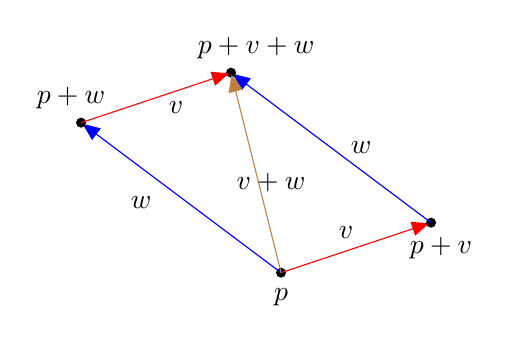
\begin{tikzpicture}[x=0.25in,y=0.25in]
\begin{scope}[>=triangle 45,shorten >=0.01in]

    \fill[black] (0,0) circle(0.1) + (+0.0,-0.5) node[black]{$p$};

    \draw[red,->] (0,0) -- (+3,+1);
    \draw[black] (1.3,0.8) node{$v$};
    \fill[black] (+3,+1) circle(0.1) + (+0.2,-0.5) node[black]{$p+v$};
    \draw[blue,->] (+3,+1) -- (-1,+4);
    \draw[black] (+1.6,2.5) node{$w$};
    \fill[black] (-1,+4) circle(0.1) + (+0.5,+0.5) node[black]{$p+v+w$};

    \draw[blue,->] (0,0) -- (-4,+3);
    \draw[black] (-2.8,1.4) node{$w$};
    \fill[black] (-4,+3) circle(0.1) + (-0.2,+0.5) node[black]{$p+w$};
    \draw[red,->] (-4,+3) -- (-1,+4);
    \draw[black] (-2.1,3.3) node{$v$};

    \draw[brown,->] (0,0) -- (-1,+4);
    \draw[black] (-0.2,1.8) node{$v+w$};
\end{scope}
\end{tikzpicture}
\end{wrapfigure}
We will define the \key{vector sum} of vectors $v=(v_x,v_y)$ and
$w=(w_x,w_y)$ to be $v+w=(v_x+w_x,v_y+w_y)$.  If you
think of a point $p=(p_x,p_y)$ in the XY-plane as a vector,
you can associate a translation $\tau_v$ of the XY-plane
with the vector $v$ using the equation $\tau_v(p)=p+v$.  Then\\
\hspace*{0.2in}$\tau_w(\tau_v(p)) = p+v+w = \tau_{v+w}(p)$ \\
See the picture.
\\[1ex]
Note that vector sums are commutative, i.e.,  $v+w=w+v$, and associative,
i.e., $u+(v+w)=(u+v)+w$.
\end{minipage}

\bigskip

\begin{minipage}{\textwidth}\raggedright
\begin{wrapfigure}{r}{0.55\textwidth}
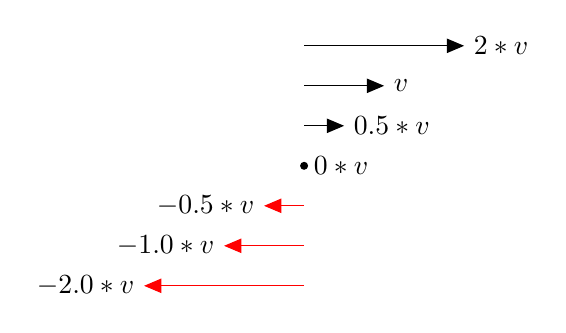
\begin{tikzpicture}[x=0.20in,y=0.20in]
\begin{scope}[>=triangle 45]

    \draw[black,->] (0,3) -- (4,3) node[black,right]{$2*v$};
    \draw[black,->] (0,2) -- (2,2) node[black,right]{$v$};
    \draw[black,->] (0,1) -- (1,1) node[black,right]{$0.5*v$};
    \fill[black] (0,0) circle(0.1) node[black,right]{$0*v$}; 
    \draw[red,->] (0,-1) -- (-1,-1) node[black,left]{$-0.5*v$};
    \draw[red,->] (0,-2) -- (-2,-2) node[black,left]{$-1.0*v$};
    \draw[red,->] (0,-3) -- (-4,-3) node[black,left]{$-2.0*v$};
\end{scope}
\end{tikzpicture}
\end{wrapfigure}
We define the \key{scalar product} of a scalar $s$ and a vector
$v=(v_x,v_y)$ as $s*v = (s*v_x,s*v,y)$.  Multiplication
of $v$ by $s>0$ does not change the direction of $v$,
but multiplies the length of $v$ by $s$.  Multiplication of $v$ by
$s<0$ reverses the direction of $v$ and multiplies its length
by $|s|$.  See the picture.
\\[1ex]
Note that scalar products are associative in the sense that
$s_1*(s_2*v)=(s_1*s_2)*v$.
\end{minipage}

\bigskip

\begin{minipage}{\textwidth}\raggedright
\begin{wrapfigure}{r}{0.4\textwidth}
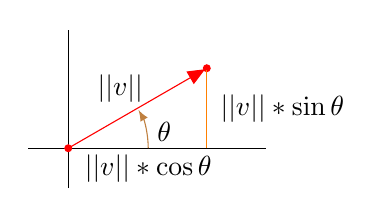
\begin{tikzpicture}[x=0.20in,y=0.20in]
\begin{scope}[>=triangle 45,shorten >=0.01in]
    \draw[black] (-1,0) -- (+5,0);
    \draw[black] (0,-1) -- (0,+3);

    \fill[red] (0,0) circle(0.1);
    \draw[black] (2.0,-0.5) node{$||v||*\cos \theta$};

    \draw[brown,>=latex,->] (2.0,0) arc(0:30:2.0);
    \draw[black] (2.4,+0.4) node{$\theta$};

    \fill[red] (3.464101615,2.0) circle(0.1);
    \draw[red,->] (0,0) -- (3.464101615,2.0);
    \draw[black] (1.3,+1.5) node{$||v||$};

    \draw[orange] (3.464101615,0) -- (3.464101615,2.0);
    \draw[black] (3.464101615,1) + (0.1,0)
                 node[right]{$||v||*\sin \theta$};
\end{scope}
\end{tikzpicture}
\end{wrapfigure}
A vector $v=(v_x,v_y)$ has a length and a direction.
The \key{length}, denoted by $||v||$, can be computed using
Pythagoras's Theorm: $||v||=\sqrt{v_x^2+v_y^2}$.  The
direction is given by the counterclockwise angle $\theta$ from
the positive X-axis direction to the vector direction.
This is called the \key{azimuth} of $v$, and in computer
languages may be computed (in radians) by the {\tt atan2} function as
$\theta = \mathrm{atan2}(v_y,v_x)$ (note $v_y$ comes before $v_x$).
\\[1ex]
The vector with length $\ell$ and azimuth $\theta$ is
$(\ell \cos\theta,\ell \sin\theta)$.
See the picture.
\\[1ex]
Note that adding integer multiples of 360 to a vector's
azimuth does \underline{not} change the vector.
\end{minipage}

\newpage

\section{Vector Calculator}
Implement additions to the basic calculator for just {\em vector}
value types and the {\em operators} and {\em functions}:
\begin{center}
\begin{tabular}{l@{~~~~~}l@{~~~~~}l}
Assume: & {\tt s=}$s$, {\tt x=}$x$, {\tt y=$y$},
          {\tt l=$\ell$}, {\tt t=$\theta$}
          are scalars \\
	& {\tt v=}$(v_x,v_y)$, {\tt w=}$(w_x,w_y)$ are vectors \\
then: \\[1ex]
\tt (x,y) & returns $(x,y)$ \\
\tt s*v & returns $(s v_x, s v_y )$ \\
\tt -v & returns $( -v_x, -v_y )$, {\tt v} with direction reversed \\
\tt v+w & returns $(v_x + w_x, v_y + w_y)$ \\
\tt v-w & returns $(v_x - w_x, v_y - w_y)$ \\
\tt ||v|| & returns $\sqrt{v_x^2 + v_y^2}$ & [length] \\
\tt azm v & returns $\mathrm{atan2}(v_y,v_x)$ & [azimuth] \\
\tt l\textasciicircum t
          & returns $(\ell\cos\theta,\ell\sin\theta)$, \\
	  & the vector with length {\tt l} and azimuth {\tt t} \\
\end{tabular}
\end{center}

\begin{center}
\begin{tabular}{rl}
Sample Input File: & \file{00-vector-vec-2d.sin} \\
Sample Output File: & \file{00-vector-vec-2d.sout} \\
or: & \file{00-vector-vec-2d.ftest} \\
Submit Run File: & \file{submit-vector-vec-2d.run} \\
\end{tabular}
\end{center}

Note that the {\tt .ftest} files for this problem are identical
to the corresponding {\tt .sout} files.

You can test your program using the indicated sample input and
output and you can submit your program using the indicated submit
run file.

\subsection{Vector Coding Hints}

You should write functions to do things like vector addition,
because later you will need to do these things in other
statements and will want a function to call.  Using the following
function signatures may make it easier
for other people familiar with this problem to read your
code, should that be important.

\hspace*{0.5in}\begin{minipage}{4.0in}
\begin{verbatim}
/* C Vector Function Signatures */
void printv ( vec );
vec addv ( vec v, vec w );
vec subv ( vec v, vec w );
vec negv ( vec v );
vec zerov = { 0, 0 };
double lenv ( vec v );
double azmv ( vec v );
vec polar ( double len, double azm );
\end{verbatim}
\end{minipage}

\bigskip

\hspace*{0.5in}\begin{minipage}{4.0in}
\begin{verbatim}
// C++ Vector Function Signatures
std::ostream & operator <<
        ( std::ostream & s, vec v );
vec operator + ( vec v, vec w );
vec operator - ( vec v, vec w );
vec operator - ( vec v );
vec zerov = { 0, 0 };
double len ( vec v );
double azm ( vec v );
vec polar ( double len, double azm );
\end{verbatim}
\end{minipage}

\section{Linear Transforms}
If we let $\mathcal{R}$ denote the set of real numbers,
a.k.a., scalars, the set of all vectors is \\
\centerline{
$\mathcal{R}\times\mathcal{R}=\mathcal{R}^2
    =\{(v_x,v_y)|v_x,v_y\in \mathcal{R}\}$}

\begin{definition}\label{LINEAR-TRANSFORMATION}
A \key{linear transformation} $L$ is a continuous map
$L:\mathcal{R}^2\mapsto\mathcal{R}^2$ such that for
all vectors $v$ and $w$, $L(v+w)=L(v)+L(w)$.
\end{definition}

Some examples of linear transformations are (1) the identity map,
(2) rotations, (3) reflections about an axis, (4) scale changes
(i.e., $(v_x,v_y)\longmapsto(s_x v_x,s_y v_y)$ for scalars $s_x$
and $s_y$).


\begin{lemma}
Let $L$ be a linear transformation, $v$ and $w$ be vectors,
and $0=(0,0)$ be the zero vector.  Then $L(0)=0$,  $L(-v)=-L(v)$,
and $L(v-w) = L(v) - L(w)$.
\end{lemma}
\begin{indpar}{0.5in}
Proof: $L(0) = L(0+0)= L(0) + L(0)$ so subtracting $L(0)$
from both sides, $0=L(0)$.  $0 = L(0) = L(v-v) = L(v) + L(-v)$
so subtracting $L(v)$ from both sides $-L(v)=L(-v)$.
$L(v-w)=L(v+(-w))=L(v)+L(-w)=L(v)+(-L(w))=L(v)-L(w)$.
\end{indpar}

\begin{lemma}
Let $L$ be a linear transformation, $s$ be a scalar, and $v$ be a vector.
Then $L(s*v)=s*L(v)$.
\end{lemma}
\begin{indpar}{0.5in}
Proof: The cases $s=0,1,2,-1,-2$ follow from the previous lemma and
using induction proves the lemma for any integer $s$.  For $s=n/d$
a rational number with integers $n$ and $d$ and $d>0$, \\
\hspace*{0.1in}$n*L(v) = L(n*(d/d)*v) = L(d*(n/d)*v)=d*L((n/d)*v)$ \\
so dividing by $d$
we get $L((n/d)*v)=(n/d)*L(v)$.  For $s$ a non-rational real number,
the result follows from a continuity argument that we will leave
to the mathematicians, since computer scientists only compute
with rational numbers.
\end{indpar}

Let $L$ be a linear transformation; let $v=(v_x,v_y)$ be a vector;
let $u_x=(1,0)$ and $u_y =(0,1)$.  Then \\
\centerline{$L(v) = L(v_x*u_x+v_y*u_y)=v_x*L(u_x)+v_y*L(u_y)$.}

\begin{lemma}
Given vectors $\ell_x$ and $\ell_y$, the map
$L:(v_x,v_y)\longmapsto v_x*\ell_x+v_y*\ell_y$ is a linear
transformation.
\end{lemma}
\begin{indpar}{0.5in}
Proof: $L(v+w) = (v_x+w_x)*\ell_x+(v_y+w_y)*\ell_y
               = v_x*\ell_x+v_y*\ell_y+w_x*\ell_x+w_y*\ell_y
	       = L(v) + L(w)$.
\end{indpar}

So $L$ is determined by $\ell_x = L(u_x)$ and $\ell_y = L(u_y)$,
and there is a 1-1 correspondence between linear transformations
and vector pairs $(\ell_x,\ell_y)$.  Therefore we will represent a linear
transformation $L$ by a pair of vectors {\tt ($\ell_x$,$\ell_y$)}
and represent application of L to the vector {\tt v = ($v_x$,$v_y$)} by \\
\centerline{\tt $L(v)$ = ($\ell_x$,$\ell_y$)*($v_x$,$v_y$) =
             $v_x$*$\ell_x$+$v_y$*$\ell_y$}

Examples:
\begin{enumerate}
\item {\tt L=((1,0),(0,1))} is the identity map.
$L(v)=v_x*(1,0) + v_y*(0,1) = (v_x,0)+(0,v_y) = (v_x,v_y) = v$.
\item {\tt L=((0,1),(-1,0))} rotates vectors $90^\circ$.
Specifically, $L(u_x)=u_y$ and $L(u_y)=-u_x$ and
$L(v)=v_x*(0,1) + v_y*(-1,0) = (0,v_x)+(-v_y,0) = (-v_y,v_x)$.
\item {\tt L=((-1,0),(0,-1))} reverses the direction of a vector.
$L(v)=v_x*(-1,0) + v_y*(0,-1) = (-v_x,0)+(0,-v_y) = (-v_x,-v_y) = -v$.
\item {\tt L=((-1,0),(0,1))} reflects vectors across the Y-axis.
$L(v)=v_x*(-1,0) + v_y*(0,1) = (-v_x,0)+(0,v_y) = (-v_x,v_y)$.
\item {\tt L=(($s_x$,0),(0,$s_y$))} scales the X-axis by $s_x$ and
the Y-axis by $s_y$. \\
$L(v)=v_x*(s_x,0) + v_y*(0,s_y)
     = (s_x v_x,0)+(0,s_y v_y)= (s_x v_x, s_y v_y)$.
\end{enumerate}

Now suppose we have a scalar {\tt s}, vector {\tt v},
and two linear transformations
{\tt K = ($\ell^K_x$,$\ell^K_y$)},
{\tt L = ($\ell^L_x$,$\ell^L_y$)}.  Then we can define:
\begin{center}
\tt
\begin{tabular}{l@{~so that~}l}
s*L = (s*$\ell^L_x$,s*$\ell^L_y$)
	 & (s*L)*v = s*(L*v) \\[0.3ex]
K+L = ($\ell^K_x$+$\ell^L_x$,$\ell^K_y$+$\ell^L_y$)
	 & (K+L)*v = K*v + L*v \\[0.3ex]
K+L = ($\ell^K_x$+$\ell^L_x$,$\ell^K_y$+$\ell^L_y$)
	 & (K+L)*v = K*v + L*v \\[0.3ex]
K-L = ($\ell^K_x$-$\ell^L_x$,$\ell^K_y$-$\ell^L_y$)
	 & (K-L)*v = K*v - L*v \\[0.3ex]
-L = (-$\ell^L_x$,-$\ell^L_y$)
	 & (-L)*v = - L*v \\[0.3ex]
K*L = (K*$\ell^L_x$,K*$\ell^L_y$)
	 & (K*L)*v = K*(L*v)
\end{tabular}
\end{center}

Note that {\tt *} and {\tt +} as defined here are bi-linear
(letting {\tt J} be another linear transformation):
\begin{center}
\tt
s*(K+L) = s*K + s*L \\
(J+K)*L = J*L + K*L \\
J*(K+L) = J*K + J*L
\end{center}

Also note that {\tt K*L} is in general \underline{not equal}
to {\tt L*K}.



\newpage

\section{Linear Transform Calculator}
Implement additions to the vector calculator for just {\em linear-transform}
value types and the {\em operators} and {\em functions}:
\begin{center}
\begin{tabular}{l@{~~~~~}l@{~~~~~}l}
Assume: & {\tt s=}$s$ is a scalar \\
	& {\tt v=($v_x$,$v_y$)} and {\tt w=($w_x$,$w_y$)} are vectors \\
	& {\tt K=($\ell^K_x$,$\ell^K_y$)} and
	  {\tt L=($\ell^L_x$,$\ell^L_y$)} are linear transforms \\
then: \\[1ex]
\tt (v,w) & returns $(v,w)$ \\
\tt L*v & returns {\tt ($v_x\ell^L_x$,$v_y\ell^L_y$)} \\
\tt s*K & returns {\tt ($s\ell^L_x$,$s\ell^L_y$)} \\
\tt K+L & returns {\tt ($\ell^K_x$+$\ell^L_x$,$\ell^K_y$+$\ell^L_y$)} \\
\tt K-L & returns {\tt ($\ell^K_x$-$\ell^L_x$,$\ell^K_y$-$\ell^L_y$)} \\
\tt -L & returns {\tt (-$\ell^L_x$,-$\ell^L_y$)} \\
\tt K*L & returns {\tt (K*$\ell^L_x$,K*$\ell^L_y$)} \\
\end{tabular}
\end{center}

\begin{center}
\begin{tabular}{rl}
Sample Input File: & \file{00-linear-vec-2d.sin} \\
Sample Output File: & \file{00-linear-vec-2d.sout} \\
or: & \file{00-linear-vec-2d.ftest} \\
Submit Run File: & \file{submit-linear-vec-2d.run} \\
\end{tabular}
\end{center}

Note that the {\tt .ftest} files for this problem are identical
to the corresponding {\tt .sout} files.

You can test your program using the indicated sample input and
output and you can submit your program using the indicated submit
run file.

\section{Rotations and Reflections}
Rotations and reflections are the two kinds of linear transformations
that preserve vector lengths (i.e., $||L(v)||=||v||$).

\begin{minipage}{\textwidth}\raggedright
\begin{wrapfigure}[5]{r}{0.4\textwidth}
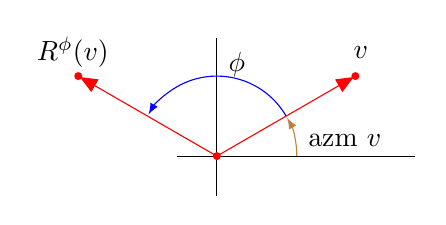
\begin{tikzpicture}[x=0.20in,y=0.20in]
\begin{scope}[>=triangle 45,shorten >=0.01in]
    \draw[black] (-1,0) -- (+5,0);
    \draw[black] (0,-1) -- (0,+3);

    \fill[red] (0,0) circle(0.1);

    \draw[brown,>=latex,->] (2.0,0) arc(0:30:2.0);
    \draw[black] (3.2,+0.4) node{azm~$v$};

    \draw[blue,>=latex,->] (1.7320508,1.0) arc(30:150:2.0);
    \draw[black] (+0.5,+2.3) node{$\phi$};

    \fill[red] (3.464101615,2.0) circle(0.1);
    \draw[red,->] (0,0) -- (3.464101615,2.0);
    \draw[black] (3.6,2.6) node{$v$};

    \fill[red] (-3.464101615,2.0) circle(0.1);
    \draw[red,->] (0,0) -- (-3.464101615,2.0);
    \draw[black] (-3.6,+2.6) node{$R^\phi(v)$};

\end{scope}
\end{tikzpicture}
\end{wrapfigure}
A rotation $R^\phi$ by $\phi$ degrees (counter-\EOL clockwise)
is defined mathematically by
\hspace*{0.2in}\begin{tabular}[t]{l}
$||R^\phi(v)|| = ||v||$ \\
$\mathrm{azm}~R^\phi(v) = \mathrm{azm}~v + \phi$ \\
\end{tabular}
\\[1ex]
Note that adding integer multiples of 360 to $\phi$
does \underline{not} change $R^\phi$.
\end{minipage}

\begin{minipage}{\textwidth}\raggedright
\begin{wrapfigure}[5]{r}{0.5\textwidth}
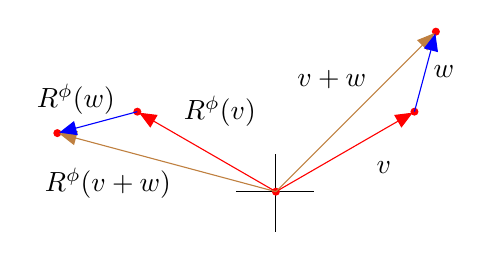
\begin{tikzpicture}[x=0.20in,y=0.20in]
\begin{scope}[>=triangle 45,shorten >=0.01in]
    \draw[black] (-1,0) -- (+1,0);
    \draw[black] (0,-1) -- (0,+1);

    \fill[red] (0,0) circle(0.1);

    \fill[red] (3.464101615,2.0) circle(0.1);
    \draw[red,->] (0,0) -- (3.464101615,2.0);
    \draw[black] (2.7,0.6) node{$v$};

    \fill[red] (4.0,4.0) circle(0.1);
    \draw[brown,->] (0,0) -- (4.0,4.0);
    \draw[black] (1.4,2.8) node{$v+w$};

    \draw[blue,->] (3.464101615,2.0) -- (4.0,4.0);
    \draw[black] (4.2,3.0) node{$w$};

    \fill[red] (-3.464101615,2.0) circle(0.1);
    \draw[red,->] (0,0) -- (-3.464101615,2.0);
    \draw[black] (-1.4,+2.0) node{$R^\phi(v)$};

    \fill[red] (-5.464101521,1.464101590) circle(0.1);
    \draw[brown,->] (0,0) -- (-5.464101521,1.464101590);
    \draw[black] (-4.2,+0.2) node{$R^\phi(v+w)$};

    \draw[blue,->] (-3.464101615,2.0) -- (-5.464101521,1.464101590);
    \draw[black] (-5.0,2.3) node{$R^\phi(w)$};

\end{scope}
\end{tikzpicture}
\end{wrapfigure}
A rotation perserves side-lengths and angles of a triangle.
Therefore, a rotation preserves vector addition, that is,
$R^\phi(v+w)=R^\phi(v)+R^\phi(w)$, and thus
satisfies Definition~\ref{LINEAR-TRANSFORMATION}
and is a linear transformation.
\end{minipage}

\newpage

\section{Products, Rotations, and Reflections}
There are two products of a pair of vectors that play a
very important role in 2D computational geometry:

\begin{definition}
The \key{scalar product} of two vectors \\
\centerline{{\tt v = ($v_x$,$v_y$)} and {\tt w = ($w_x$,$w_y$)}} \\
is \\
\centerline{\tt v*w = $v_x w_x + v_y w_y$} \\
The \key{cross product} of the two vectors is \\
\centerline{\tt v\#w = $v_x(-w_y) + v_y w_x$}
\end{definition}

Above we denoted the length of a vector {\tt v} by {\tt ||v||}.
Then \\
\centerline{\tt ||v||$^2$ = v*v}

Let us denote the vector {\tt w} rotated counter-clockwise by
{\tt d} degrees by {\tt w\textasciicircum d}.  Then \\
\centerline{\tt v\#w = v*(w\textasciicircum 90)}

\begin{lemma}
Both the scalar and cross product are \key{bi-linear}.  That is,
if {\tt u}, {\tt v}, {\tt w} are vectors and {\tt s} is a scalar:
\begin{center}
\tt
(u+v)*w = u*w + v*w \\
u*(v+w) = u*v + u*w \\
(s*u)*w = s*(u*w) = u*(s*w) \\
(u+v)\#w = u\#w + v\#w \\
u\#(v+w) = u\#v + u\#w \\
(s*u)\#w = s*(u\#w) = u\#(s*w)
\end{center}

\end{lemma}

Note that the scalar product is symmetric ({\tt v*w = w*v})
while the cross produce is anti-symmetric ({\tt v\#w = -w\#v}).

\begin{definition}
A linear transformation {\tt L} is \key{unitary} if and only if
{\tt L(v)*L(w) = v*w} for every pair of vectors {\tt v} and {\tt w}
({\tt L} preserves scalar products).

A unitary transformation is a \key{rotation} if and only if
{\tt L(v)\#L(w) = v\#w} for every pair of vectors {\tt v} and {\tt w}.

A unitary transformation is a \key{reflection} if and only if
{\tt L(v)\#L(w) = - v\#w} for every pair of vectors {\tt v} and {\tt w}.

\end{definition}

\begin{lemma}
A linear transformation {\tt L = ($\ell_x$,$\ell_y$)} is unitary
if and only if \\
\centerline{{\tt ||$\ell_x$||=1}, {\tt ||$\ell_y$||=1}, and
{\tt $\ell_x$*$\ell_y$=0}}

{\tt L} is a rotation if and only if it is unitary and
{\tt $\ell_x$\#$\ell_y$=-1}.

{\tt L} is a reflection if and only if it is unitary and
{\tt $\ell_x$\#$\ell_y$=1}.
\end{lemma}
\begin{indpar}{0.5in}
Proof:  Let {\tt $u_x$ = (1,0)} and {\tt $u_y$ = (0,1)} so
that {\tt $\ell_x$ = L($u_x$)} and {\tt $\ell_y$ = L($u_y$)}.
Then {\tt $u_x$*$u_x$ = 1}, {\tt $u_y$*$u_y$ = 1}, {\tt $u_x$*$u_y$ = 0},
and {\tt $u_x$\#$u_x$ = 0}, {\tt $u_y$\#$u_y$ = 0}, {\tt $u_x$\#$u_y$ = -1}.

Then if {\tt L} is unitary, \\
\hspace*{0.1in}
{\tt L($u_x$)*L($u_x$) = 1}; {\tt L($u_y$)*L($u_y$) = 1};
{\tt L($u_x$)*L($u_y$) = 0} \\
If in addition it is a rotation, 
{\tt L($u_x$)\#L($u_y$) = -1}, while if instead it is a reflection,
{\tt L($u_x$)\#L($u_y$) = 1}.

Conversely, if we assume {\tt ||$\ell_x$|| = 1}, etc., then the
converse follows from:
\begin{center}
\tt
\begin{tabular}{r@{~=~}l}
L(v)*L(w) & L($v_x$*$u_x$+$v_y$*$u_y$)*L($w_x$*$u_x$+$w_y$*$u_y$) \\
	  & $v_x w_x$*L($u_x$)*L($u_x$)
	    \begin{tabular}[t]{@{}l}
	    + $v_x w_y$*L($u_x$)*L($u_y$) \\
	    + $v_y w_x$*L($u_y$)*L($u_x$) \\
	    + $v_y w_y$*L($u_y$)*L($u_y$) \\
	    \end{tabular} \\
	  & $v_x w_x$ + 0 + 0 + $v_y w_y$ \\
	  & v*w
\\[1ex]
L(v)\#L(w) & L($v_x$*$u_x$+$v_y$*$u_y$)\#L($w_x$*$u_x$+$w_y$*$u_y$) \\
	  & $v_x w_x$*L($u_x$)\#L($u_x$)
	    \begin{tabular}[t]{@{}l}
	    + $v_x w_y$*L($u_x$)\#L($u_y$) \\
	    + $v_y w_x$*L($u_y$)\#L($u_x$) \\
	    + $v_y w_y$*L($u_y$)\#L($u_y$) \\
	    \end{tabular} \\
	  & 0 $\mp$ $v_x w_y$ $\pm$ $v_y w_x$ + 0 \\
	  & $\pm$ v\#w
\end{tabular}
\end{center}
\end{indpar}

\begin{lemma}
A unitary linear transformation (in 2 dimensions)
is either a rotation or a reflection.
\end{lemma}
\begin{indpar}{0.5in}
Proof: By laborious algebra we prove the {\tt v*w = 0} implies
{\tt |v\#w| = ||v||*||w||} which for a unitary transformation
{\tt ($\ell_x$,$\ell_y$)} implies that {\tt |$\ell_x$\#$\ell_y$| = 1},
so by the last lemma we are done.  The laborious algebra is:
\begin{center}
\begin{tabular}{r@{~=~}l}
\tt |v\#w|$^2$ & $(v_x(-w_y)+v_y w_x)^2$ \\
               & $v_x^2 w_y^2 - 2 v_x v_y w_x w_y + v_y^2 w_x^2$ \\
\tt (||v||*||w||)$^2$
               & $(v_x^2+v_y^2)(w_x^2+w_y^2)$ \\
               & $v_x^2 w_y^2 + v_x^2 w_x^2 + v_y^2 w_y^2 + v_y^2 w_x^2$ \\
and using      & $v_x w_x + v_y w_y = 0$ \\
$v_x^2 w_x^2$  & $v_x^2 w_x^2 - (v_x w_x + v_y w_y)v_x w_x$ \\
	       & $-v_x v_y w_x w_y$ \\
$v_y^2 w_y^2$  & $v_y^2 w_y^2 - (v_x w_x + v_y w_y)v_y w_y$ \\
	       & $-v_x v_y w_x w_y$ \\
\end{tabular}
\end{center}
\end{indpar}

\section{Unitary Transform Calculator}
Add the linear transformation value to your calculator and implement
the following {\em operators} and {\em functions}:
\begin{center}
\begin{tabular}{l@{~~~~~}l@{~~~~~}l}
Assume: & {\tt d=}$d$ (a scalar) \\
	& {\tt v=}$(v_x,v_y)$ (a vector) \\
	& {\tt w=}$(w_x,w_y)$ (a vector) \\
then: \\[1ex]
\tt v*w & returns $v_x w_x + w_y w_y$,
          the scalar product of {\tt v} and {\tt w} \\
\tt v\#w & returns $v_x(-w_y)+v_y w_x$,
           the cross product of {\tt v} and {\tt w} \\
\tt v\textasciicircum d & returns {\tt v} rotated counter-clockwise by
			  $d$ degrees \\

TBD
\end{tabular}
\end{center}

\begin{center}
\begin{tabular}{rl}
Sample Input File: & \file{00-unitary-vec-2d.sin} \\
Sample Output File: & \file{00-unitary-vec-2d.sout} \\
or: & \file{00-unitary-vec-2d.ftest} \\
Submit Run File: & \file{submit-unitary-vec-2d.run} \\
\end{tabular}
\end{center}

Note that the {\tt .ftest} files for this problem are identical
to the corresponding {\tt .sout} files.

You can test your program using the indicated sample input and
output and you can submit your program using the indicated submit
run file.


\bigskip

\begin{tabular}{ll}
Author:	      & Robert L.~Walton $<$walton@acm.org$>$ \\
Date:         & Mon Oct 19 11:25:00 EDT 2020
\end{tabular}

The authors have placed this problem in the public domain;
they make no warranty and accept no liability for this problem.

\end{document}
